\documentclass[12pt,article,twosided]{memoir}
%% ::: Memoir class options for page size
%% ::: * the STOCK SIZE is LETTER
%% ::: * the TRIMMED SIZE is 6 x 9
\setlrmarginsandblock{1.25in}{*}{1}
\setulmarginsandblock{1.75in}{*}{1}
\setheadfoot{0.55in}{0.75in}
\checkandfixthelayout

\usepackage{polyglossia}
\setdefaultlanguage{english}
\setotherlanguage{sanskrit}
\setotherlanguage{tamil}
\setotherlanguage{telugu}
\setotherlanguage{kannada}
\setotherlanguage{malayalam}
\defaultfontfeatures{Mapping=tex-text}
\setmainfont[Numbers={Proportional},SmallCapsFont={Adobe Caslon Pro},SmallCapsFeatures={Letters=SmallCaps,Numbers=Lining}]{Adobe Caslon Pro}
\newfontfamily\tamilfont[Script=Tamil]{AksharUnicodeRegular}
\newfontfamily\sanskritfont[Script=Devanagari]{Jaini}
\newfontfamily\greekfont[Script=Greek]{GFS Porson}
\usepackage[shortcuts]{extdash}
\usepackage{tikz}
\usetikzlibrary{backgrounds, matrix, positioning, fadings, through}
\usepackage{pgf}
\usepackage{tipa}
\usepackage{fontawesome5}
\usepackage{calc}
\usepackage{natbib}
	\bibpunct[: ]{(}{)}{; }{a}{ }{,}
\usepackage{xcolor}
\definecolor{Nesarlink}{HTML}{f6820b}
\definecolor{Nesarlinkdark}{HTML}{8a4b0b}
\definecolor{Nesarlinklight}{HTML}{fff0e0}
\usepackage{catchfile}
\usepackage{graphicx,graphbox}
\graphicspath{{images/}}
\usepackage{ragged2e}
\usepackage{changepage}
\usepackage{trimspaces}
\usepackage{framed}
\usepackage[most]{tcolorbox}
\usepackage[bottom,marginal,multiple]{footmisc}
\def\changemargin#1#2{\list{}{\rightmargin#2\leftmargin#1}\item[]}
\let\endchangemargin=\endlist 
\makeatletter
\renewcommand\@makefntext[1]{%
  \par \parindent=\z@ \noindent
  \llap{\@thefnmark.\quad}%
  {\addfontfeatures{Numbers=Lining}#1}%
}
\CatchFileDef\slug{metadata-slug.tex}{}
\CatchFileDef\doi{metadata-doi.tex}{}
\CatchFileDef\Ndate{metadata-date.tex}{}
\CatchFileDef\citation{metadata-citation.tex}{}
\makeatother
\def\trim#1{\ignorespaces#1\unskip}
\newcommand{\Nyear}{\trim{2022}}
\newcommand{\Nauthor}{\trim{Jonathan Peterson}}
\newcommand{\Ntitle}{\trim{Meat Matters}}
\newcommand{\article}{\trim{1}}
\newcommand{\issue}{\trim{0}}
%\CatchFileDef\Nyear{year.tex}{}
%\CatchFileDef\article{article.tex}{}
%\CatchFileDef\issue{issue.tex}{}
\makeatother
\title{\protect\Ntitle}
\author{\protect\Nauthor}
\newcommand{\oldnums}[1]{{\fontspec[Numbers={Proportional,OldStyle}]{Adobe Caslon Pro}#1}}
\newcommand{\oldnumsbold}[1]{{\fontspec[Numbers={Proportional,OldStyle}]{Adobe Caslon Pro}\textbf{#1}}}
\setsecnumformat{\csname #1secnumformat\endcsname}
\newcommand\sectionsecnumformat{\oldnumsbold{\thesection}\quad }
\newcommand\onpage{\oldnums{\thepage}}

% Button for CC 4.0 BY
\newcommand{\ccbylicenseButton}{%
\href{https://creativecommons.org/licenses/by/4.0/}{
\includegraphics[align=t,width=2cm]{byNesar.png}}}
% Link to journal
\newcommand{\journallink}{%
\expandafter\url\expandafter{https://nesarjournal.org/articles/\expandafter\slug}}
% Link to DOI
\newcommand{\doilink}{%
\expandafter\url\expandafter{https://doi.org/\expandafter\doi}}
% Issue.Article (Year)
\newcommand{\iay}{%
\fontspec[Numbers={Proportional,OldStyle}]{TeX Gyre TermesX}\issue.\article\ (\Nyear)}
% Journal logo and link
\newcommand{\brand}{%

\includegraphics[width=0.5cm,align=c]{logoNesardark.png} \hspace{0.25em} \href{https://nesarjournal.org}{\color{Nesarlinkdark}{\emph{New Explorations in South Asia Research}}}}
% Short author name (small caps, last name)
\newcommand{\shauthor}{\textsc{steinschneider}}
\newcommand\picon[1]{\raisebox{0ex}{\footnotesize{\fontspec{Printers Ornaments One}#1}}}

\makepagestyle{firstpage}
\makeevenfoot{firstpage}{\footnotesize\begin{tabular}[b]{l}%
© \theauthor – \emph{New Explorations in South Asia Research} – \Ndate\\
\journallink\\
\doilink\end{tabular}}{}{\ccbylicenseButton\vfill}
\makeoddfoot{firstpage}{\footnotesize\begin{tabular}[b]{l}%
© \theauthor – \emph{New Explorations in South Asia Research} – \Ndate\\
\journallink\\
\doilink\end{tabular}}{}{\ccbylicenseButton\vfill}

\makepagestyle{finalpage}
\makeevenfoot{finalpage}{}{}{}
\makeoddfoot{finalpage}{}{}{}
\makeevenhead{finalpage}{}{}{\onpage}
\makeoddhead{finalpage}{\onpage}{}{}

\newcommand{\footer}{%
\begingroup\vfill\vspace{4ex}\noindent\begin{minipage}[t]{0.3\textwidth}
\noindent
\includegraphics[align=t,width=0.975\textwidth]{logo-wordmark.png}\\[1ex]
\resizebox{0.975\textwidth}{!}{\href{https://nesarjournal.org}{\color{Nesarlinkdark}{\texttt{https://nesarjournal.org}}}}
\end{minipage}\hfill
\begin{minipage}[t]{0.6\textwidth}
\footnotesize\raggedright\noindent{}\citation
\end{minipage}\endgroup}

\createmark{section}{both}{nonumber}{}{}
\nouppercaseheads
\makepagestyle{nesar}
\makeevenhead{nesar}{}{}{\color{Nesarlinkdark}{\thetitle \hspace{0.25em} \picon{e} \hspace{0.25em} \onpage}}
\makeoddfoot{nesar}{\brand\  \iay}{}{}
\makeevenfoot{nesar}{}{}{}
\makeoddhead{nesar}{\color{Nesarlinkdark}{\onpage \hspace{0.35em} \reflectbox{\picon{e}} \hspace{0.25em} \shauthor}}{}{}
\newtcolorbox{titlebox}[1][]{
    enhanced,
    boxrule=2pt,
    colframe=Nesarlinkdark!50!black,
    rounded corners,
    fontupper=\rmfamily,
    colback=Nesarlinklight!50!white,
    #1
    }

\newlength\drop
\newcommand*\titleM
  {%
    \begingroup
    \begin{tikzpicture}[remember picture, overlay]
      \path [bottom color = Nesarlink, top color = white, ] (current page.south west) rectangle ([yshift=-5cm]current page.east);   % Adjust the position of the logo.
    \end{tikzpicture}
    \noindent \emph{An offprint from}\bigskip

    
\includegraphics[width=0.65\textwidth]{logo-wordmark.png}
%    \AddToShipoutPictureBG*
%      {%
%        \AtPageLowerLeft
%          {%
%            \includegraphics[width=\paperwidth,height=\paperheight]
%              {example-image-duck}%
%          }%
%      }%
    \setlength\drop{0.15\textheight}%
    \begin{center}%
    \vspace*{\drop}%
    \begin{tikzpicture}[remember picture, overlay]
      \node[inner sep=0pt] (backgroundimage) at ([yshift=-2cm]current page.center) {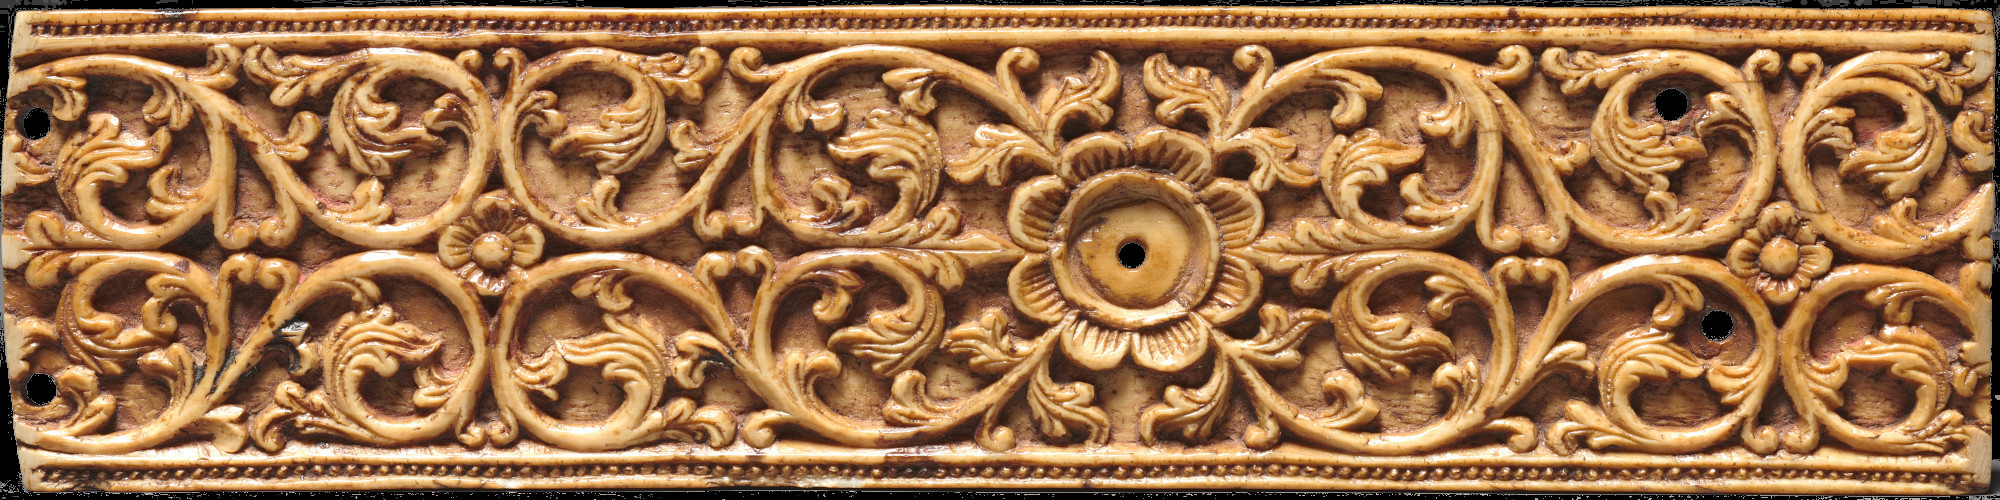
\includegraphics[width=1.2\paperwidth]{ollett-introducing-nesar.jpg}};
      \node[inner sep=0pt] (titlebox) at ([yshift=0.55cm]backgroundimage.north) {\begin{titlebox}\begin{center}\vspace{2ex}%
          {\HUGE\thetitle\par}\vspace{1.5ex}%
          {\Large\textit\theauthor\par}\vspace{2ex}% 
          \end{center}\end{titlebox}};
      \node[inner sep=0pt] (caption) at ([yshift=1cm,xshift=-4.75cm]current page.south east) {\begin{titlebox}[add to width=-6.5cm,fontupper=\linespread{0.75}\selectfont
]%
          {\tiny\raggedright \emph{image source}: Ivory Cover of a Palm-Leaf Manuscript, Sri Lanka, 1600s, Cleveland Museum of Art (via \href{https://commons.wikimedia.org/wiki/File:Ceylon,_17th_century_-_Cover_of_a_Palm-Leaf_Manuscript_-_1992.85_-_Cleveland_Museum_of_Art.tif}{Wikimedia Commons})}%
          \end{titlebox}};

    \end{tikzpicture}
    \vfill
    %{\Large\scshape\press}%
    \end{center}%
    
    \endgroup
  }


\usepackage[linguistics]{forest}
\usepackage{pgfornament}
\usepackage{booktabs,multirow}
\usepackage{wrapfig}
\usepackage{enumitem}
\setlist[itemize]{labelindent=\parindent,itemsep=0.15em,topsep=0pt,leftmargin=\parindent}
\counterwithout{section}{chapter}
\setsecnumdepth{subsubsection}
\maxtocdepth{subsubsection}
\setlength{\cftsectionindent}{1em}
\setlength{\cftsubsectionindent}{1em}
\setlength{\cftsubsubsectionindent}{1em}
\setlength{\parindent}{2em}
\renewcommand{\cftsectionfont}{\bfseries}
\newcommand{\longmark}{{\fontspec{EB Garamond}\raisebox{0.3ex}{ː}\hspace{0.1em}}}
\newcommand{\graph}[1]{{\fontspec{Linux Libertine O}〈#1〉}}
\newcommand{\textgreek}[1]{{\fontspec{GFS Porson}#1}}
\newcommand{\phonet}[1]{{\fontspec{Linux Libertine O}\lbrack#1\rbrack}}
\newcommand{\phonem}[1]{{\fontspec{Linux Libertine O}/#1/}}
\newcommand{\mora}{{\fontspec{GFS Porson}μ}}
\newcommand{\syll}{{\fontspec{GFS Porson}σ}}
\renewcommand{\baselinestretch}{1.1}
\setlength{\RaggedRightParindent}{\parindent}


\definecolor{formalshade}{rgb}{0.95,0.95,1}
\definecolor{darkblue}{rgb}{0.0, 0.0, 0.55}
\newtcolorbox{pullquote}{
    enhanced,
    boxrule=0pt,
    frame hidden,
    borderline west={2pt}{0pt}{Nesarlinkdark},
    colback=Nesarlinklight,
    sharp corners,
    fontupper=\rmfamily,
    left skip=24pt
    }

\usepackage{hyperref}
\hypersetup{pdftitle={\protect\input{title}},
        colorlinks,
        urlcolor=Nesarlink,
        linkcolor=Nesarlink} 

\DeclareRobustCommand{\thinskip}{\hskip 0.16667em\relax}
\def\emdash{—}
\def\d@sh#1#2{\unskip#1\thinskip#2\thinskip\ignorespaces}
\def\Dash{\d@sh\nobreak\emdash}
\def\Ldash{\d@sh\empty{\hbox{\emdash}\nobreak}}
\def\Rdash{\d@sh\nobreak\emdash}

\newcounter{excounter}
\setcounter{excounter}{1}
\newenvironment{exe}[1]{
\begin{changemargin}{2em}{0em}\noindent\textbf{\theexcounter.\ \ #1}
\end{changemargin}
\begin{changemargin}{4em}{0em}\vspace{-1ex}\noindent\ignorespaces}%
{\end{changemargin}\addtocounter{excounter}{1}}

%\usepackage[en]{metre}
%\usepackage{gb4e}
\begin{document}
%\RaggedRight

\thispagestyle{empty}
\titleM
\clearpage

\thispagestyle{empty}
\begingroup
\small

\noindent\begin{minipage}[t]{0.8\textwidth}
\noindent\textbf{NEW EXPLORATIONS IN SOUTH ASIA RESEARCH (NESAR)}\smallskip

\noindent An open-access journal of South Asian Studies, founded in 2022.\medskip

\noindent ISSN 2834-3875 \hspace{0.25em} 
\includegraphics[width=0.45cm,align=c]{logoNesar.png} \hspace{0.25em} \url{https://nesarjournal.org}\medskip

\noindent This PDF was generated \today.
\end{minipage}
\begin{minipage}[t]{0.2\textwidth}

\includegraphics[align=t,width=0.5cm]{openaccess.png}
\end{minipage}

\bigskip\bigskip

\noindent\emph{Editorial board}:\smallskip

\noindent\begin{itemize}[itemsep=2pt,parsep=0pt,leftmargin=0.45cm,label={}]
\item Andrew \textsc{OLLETT}, University of Chicago
\item Shubha \textsc{SHANTHAMURTHY}
\item Naresh \textsc{KEERTHI}, Ashoka University
\end{itemize}\medskip

\noindent\emph{Advisory board}:\smallskip

\noindent\begin{itemize}[itemsep=2pt,parsep=0pt,leftmargin=0.45cm,label={}]
\item Diwakar \textsc{ACHARYA}, University of Oxford
\item Richard \textsc{EATON}, University of Arizona
\item Leslie \textsc{ORR}, Concordia University
\item David \textsc{SHULMAN}, Hebrew University of Jerusalem
\item Eva \textsc{WILDEN}, University of Hamburg
\end{itemize}\medskip

\noindent\emph{Principal contact}:\smallskip

\noindent\hspace{0.45cm}Andrew \textsc{OLLETT} (\href{mailto:ollett@uchicago.edu}{\texttt{\color{Nesarlink}ollett@uchicago.edu}})\bigskip\bigskip

\noindent\begin{minipage}[t]{0.48\textwidth}
\begingroup
\tiny\raggedright\noindent
This article is available under a \href{https://creativecommons.org/licenses/by/4.0/}{CC BY 4.0} license. You are free to: 
\begin{itemize}[leftmargin=0.35cm,parsep=0pt,itemsep=0pt]
\item \textbf{Share}: copy and redistribute the material in any medium or format
\item \textbf{Adapt}: remix, transform, and build upon the material for any purpose, even commercially.
\end{itemize}
\noindent under the following terms:
\begin{itemize}[leftmargin=0.35cm,parsep=0pt,itemsep=0pt]
\item \textbf{Attribution}: You must give appropriate credit, provide a link to the license, and indicate if changes were made. You may do so in any reasonable manner, but not in any way that suggests the licensor endorses you or your use.
\item \textbf{No additional restrictions}: You may not apply legal terms or technological measures that legally restrict others from doing anything the license permits.
\end{itemize}\smallskip

\begin{center}

\includegraphics[align=t,width=2cm]{byNesar.png}
\end{center}\smallskip

\tiny\noindent The copyright of this article, as well as all moral rights, rest with the author (\theauthor{}).\vfill

\endgroup
\bigskip
\end{minipage}\hfill
\begin{minipage}[t]{0.48\textwidth}
\begingroup
\tiny
\noindent This PDF file was generated automatically from a source in \href{https://tei-c.org/}{TEI} encoding. The stylesheets used for the transformation are available on \href{https://github.com/nesar-journal/nesar-stylesheets}{this GitHub website}.\medskip

\noindent NESAR uses the \href{https://bombay.indology.info/software/fonts/induni/index.html}{IndUni fonts} designed by John Smith.\medskip

\begin{center}

\includegraphics[width=0.75\textwidth,align=t]{cosas.png}\medskip


\includegraphics[width=0.75\textwidth,align=t]{library.png}
\end{center}\medskip

\noindent NESAR gratefully acknowledges the support of the \href{https://www.lib.uchicago.edu/}{University of Chicago Libraries} and the \href{https://southernasia.uchicago.edu/}{Committee on Southern Asian Studies at the University of Chicago}.\vfill

\endgroup
\end{minipage}
\endgroup
\setcounter{page}{0}
\clearpage

\begin{center}{\noindent\huge{\thetitle}}\bigskip\bigskip

\begin{tabular}{c}
Andrew Ollett\\[2ex]
{\small\emph{University of Chicago}}\\[1ex]
{\small\href{mailto:ollett@uchicago.edu}{\texttt{ollett@uchicago.edu}}}
\end{tabular}
\end{center}



\begin{KeepFromToc}
  {\small 
  \tableofcontents 
}
\end{KeepFromToc}\bigskip

\pagestyle{nesar}

